%%%%%%%%%%%%%%%%%%%%%%%%%%%%%%%%%%%%%%%%%
% Beamer Presentation
% LaTeX Template
% Version 1.0 (10/11/12)
%
% This template has been downloaded from:
% http://www.LaTeXTemplates.com
%
% License:
% CC BY-NC-SA 3.0 (http://creativecommons.org/licenses/by-nc-sa/3.0/)
%
%%%%%%%%%%%%%%%%%%%%%%%%%%%%%%%%%%%%%%%%%

%----------------------------------------------------------------------------------------
%	PACKAGES AND THEMES
%----------------------------------------------------------------------------------------

\documentclass{beamer}

\mode<presentation> {

% The Beamer class comes with a number of default slide themes
% which change the colors and layouts of slides. Below this is a list
% of all the themes, uncomment each in turn to see what they look like.

%\usetheme{default}
%\usetheme{AnnArbor}
%\usetheme{Antibes}
%\usetheme{Bergen}
%\usetheme{Berkeley}
%\usetheme{Berlin}
%\usetheme{Boadilla}
\usetheme{CambridgeUS}
%\usetheme{Copenhagen}
%\usetheme{Darmstadt}
%\usetheme{Dresden}
%\usetheme{Frankfurt}
%\usetheme{Goettingen}
%\usetheme{Hannover}
%\usetheme{Ilmenau}
%\usetheme{JuanLesPins}
%\usetheme{Luebeck}
%\usetheme{Madrid}
%\usetheme{Malmoe}
%\usetheme{Marburg}
%\usetheme{Montpellier}
%\usetheme{PaloAlto}
%\usetheme{Pittsburgh}
%\usetheme{Rochester}
%\usetheme{Singapore}
%\usetheme{Szeged}
%\usetheme{Warsaw}

% As well as themes, the Beamer class has a number of color themes
% for any slide theme. Uncomment each of these in turn to see how it
% changes the colors of your current slide theme.

%\usecolortheme{albatross}
\usecolortheme{beaver}
%\usecolortheme{beetle}
%\usecolortheme{crane}
%\usecolortheme{dolphin}
%\usecolortheme{dove}
%\usecolortheme{fly}
%\usecolortheme{lily}
%\usecolortheme{orchid}
%\usecolortheme{rose}
%\usecolortheme{seagull}
%\usecolortheme{seahorse}
%\usecolortheme{whale}
%\usecolortheme{wolverine}

%\setbeamertemplate{footline} % To remove the footer line in all slides uncomment this line
%\setbeamertemplate{footline}[page number] % To replace the footer line in all slides with a simple slide count uncomment this line

%\setbeamertemplate{navigation symbols}{} % To remove the navigation symbols from the bottom of all slides uncomment this line
}

\usepackage{graphicx} % Allows including images
\usepackage{booktabs} % Allows the use of \toprule, \midrule and \bottomrule in tables

%----------------------------------------------------------------------------------------
%	TITLE PAGE
%----------------------------------------------------------------------------------------

\title[Extreme Value in Financial Statistics]{Extreme Value in Financial Statistics} % The short title appears at the bottom of every slide, the full title is only on the title page

\author{Killian Martin--Horgassan} % Your name
\institute[EPFL] % Your institution as it will appear on the bottom of every slide, may be shorthand to save space
{
Ecole Polytechnique F\'{e}d\'{e}rale de Lausanne \\ % Your institution for the title page
\medskip
\textit{killian.martin-horgassan@epfl.ch} % Your email address
}
\date{Friday 26$^{th}$ June 2015} % Date \today, can be changed to a custom date

\begin{document}

\begin{frame}
\titlepage % Print the title page as the first slide
\end{frame}

\begin{frame}
\frametitle{Table of contents} % Table of contents slide, comment this block out to remove it
\tableofcontents % Throughout your presentation, if you choose to use \section{} and \subsection{} commands, these will automatically be printed on this slide as an overview of your presentation
\end{frame}

%----------------------------------------------------------------------------------------
%	PRESENTATION SLIDES
%----------------------------------------------------------------------------------------

%------------------------------------------------
\section{Introduction} 
% Sections can be created in order to organize your presentation into discrete blocks, all sections and subsections are automatically printed in the table of contents as an overview of the talk
%------------------------------------------------
\begin{frame}{Introduction }
	\textcolor{red}{What we have} Data about past events e.g. the record of the prices of a stock over time.\newline \\
	\textcolor{red}{What we want to know} Values taken at \underline{future extreme events} e.g. maximum price between $T$ and $T + \Delta T$.
\end{frame}

\section{The two extremal problems}
\begin{frame}{Settings}
	\textcolor{red}{Observations} $(X_n)_{n \ge 0}$ i.i.d. rvs $\sim F_X$. \newline 
	\textcolor{red}{Maxima} $(M_n)_{n \ge 0} = (\max_{0 \le i \le n}(X_i))_{n \ge 0}$ \newline
	\textcolor{red}{Standardized maxima} $(M^{*}_n)_{n \ge 0}$ = $(\frac{M_n - b_n}{a_n})_{n \ge 0}$, $a_n > 0$, $b_n \in \mathbb{R}$ \newline \\ \\
	\textbf{Convergence in distribution of $(M^{*}_n)_{n \ge 0}$ ?}
	\begin{itemize}
		\item Possible limits ? \\
		\textcolor{white}{Alinea} $\implies$ \textcolor{red}{extremal limit pb} 
		\item Under what conditions ? \\
		\textcolor{white}{Alinea} $\implies$ \textcolor{red}{domain of attraction pb} 
	\end{itemize}
	
\end{frame}

\begin{frame}{Fisher-Tippett-Gnedenko theorem}
	\frametitle{Fisher-Tippett-Gnedenko Theorem}
	\begin{theorem}[Fisher-Tippett-Gnedenko]
		If the sequence of standardized maxima converges to a non-degenerate distribution, then this distribution is either a Gumbel, a Fr\´{e}chet or a Weibull distribution .
	\end{theorem}
\end{frame}

\begin{frame}{Extreme value distributions}
	\frametitle{Extreme value distributions}
	\begin{itemize}
		\item \textbf{Fr\'{e}chet} $\Phi_\alpha(x) = \exp(- x^\alpha)$ \newline
		\item \textbf{Weibull} $\Psi_\alpha(x) = \exp(-  \lvert x \rvert^\alpha)$ \newline
		\item \textbf{Gumbel} $\Delta(x) = \exp(- \exp(- x))$
	\end{itemize}
\end{frame}

\begin{frame}{Domain of attraction}
	\begin{itemize}
		\item \textcolor{red}{Domain of attraction} of an EV distribution $\implies$ set of $F_X$ such that the standardized maxima converge to this EV distribution. \newline
		Notation : $\mathcal{D}(\cdot)$ where $\cdot = \Phi_\alpha$, $\Psi_\alpha$ or $\Delta$.
		\newline
		\item \textcolor{red}{Hazard function} \newline
		 \textcolor{white}{IndentInvisibleTextBAD} $r(x) = \frac{f_X(x)}{1 - F_X(x)}$
	\end{itemize}
\end{frame}

\begin{frame}{Von Mises' Theorem}
	\frametitle{Von Mises' Theorem}
	\begin{theorem}[Von Mises' Theorem]
		\begin{itemize}
		\item If $x^+ = + \infty$ and $x r(x) \xrightarrow[x \rightarrow + \infty]{} \alpha > 0$, then $F_X \in \mathcal{D}(\Phi_\alpha)$.
		\item If $x^+ < + \infty$ and $(x^+ - x) r(x) \xrightarrow[x \rightarrow x^+]{} \alpha > 0$, then $F_X \in \mathcal{D}(\Psi_\alpha)$.
		\item If $\exists$ neighbourhood of $x^+$ where $r(x) \ge 0$, differentiable and $\frac{\mathrm{d}r}{\mathrm{d}x}(x) \xrightarrow[x \rightarrow x^+]{} 0$, then $F_X \in \mathcal{D}(\Delta)$.
		\end{itemize}
	\end{theorem}
\end{frame}

\section{Looking into financial data}
\begin{frame}{Looking into financial data }
	Our starting point : 5 stocks listed on the Paris Stock Exchange. Stock price data over 15 years.
	\begin{center}
		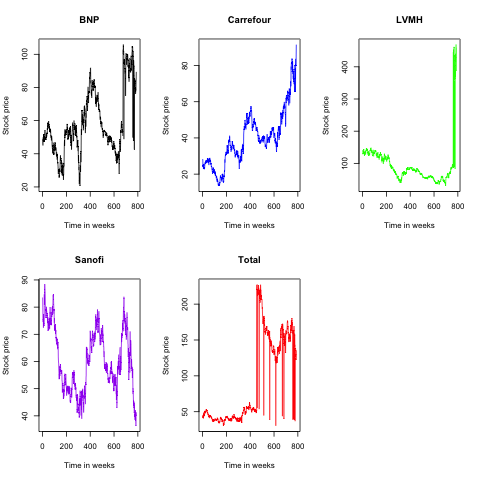
\includegraphics[scale = 0.4]{plainData.png}
	\end{center}
\end{frame}

\begin{frame}{The Black-Scholes model for stock prices}
	The price increment at time t should be proportional to the price at time t. \newline
	\textbf{SDE} : \newline \\
	\begin{cases} \mathrm{d}S_t = \mu S_t \mathrm{d}t + \sigma S_t \mathrm{d}B_t \\ 
		S(0) = s_0 \\
	 \end{cases}
	 \newline \\
	 \textbf{Solution} : \textcolor{red}{Geometric Brownian Motion} \newline
	 $S_t = s_0 \exp((\mu -\frac{\sigma^2}{2}) t + \sigma B_t)$
\end{frame}

\begin{frame}{Simulation using a GBM }
	\begin{center}
		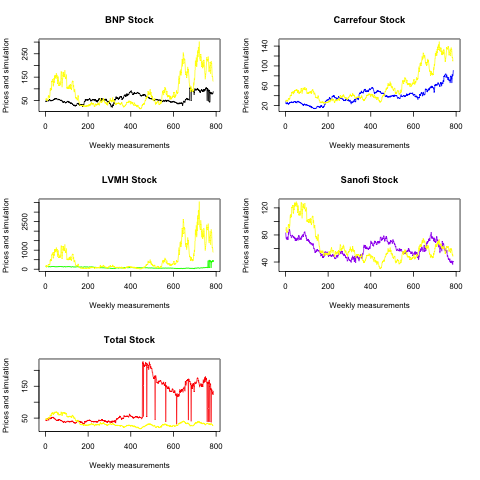
\includegraphics[scale = 0.45]{dataPlusSimulation.png}
	\end{center}
\end{frame}

\begin{frame}{Simulation using a GBM - observations}
	\begin{itemize}
		\item The simulation may overestimate \textit{wrt} to the actual prices. \\
		\item \textcolor{red}{On the whole $\implies$ rather satisfactory...} \\
		\item ... except for the LVMH and even worse the Total stocks. \\
		\item \textcolor{red}{sudden \& large variations $\implies$ model performs very poorly.}
	\end{itemize}
\end{frame}

\section{Statistics of extremes \& financial data}
\begin{frame}{Statistics of extremes \& financial data (I)}
	Making the junction
\end{frame}

%\subsection{Subsection Example} % A subsection can be created just before a set of slides with a common theme to further break down your presentation into chunks

%------------------------------------------------

%\begin{frame}
%\frametitle{Blocks of Highlighted Text}
%\begin{block}{Block 1}
%Lorem ipsum dolor sit amet, consectetur adipiscing elit. Integer lectus nisl, ultricies in feugiat rutrum, porttitor sit amet augue. Aliquam ut tortor mauris. Sed volutpat ante purus, quis accumsan dolor.
%\end{block}

%\begin{block}{Block 2}
%Pellentesque sed tellus purus. Class aptent taciti sociosqu ad litora torquent per conubia nostra, per inceptos himenaeos. Vestibulum quis magna at risus dictum tempor eu vitae velit.
%\end{block}

%\begin{block}{Block 3}
%Suspendisse tincidunt sagittis gravida. Curabitur condimentum, enim sed venenatis rutrum, ipsum neque consectetur orci, sed blandit justo nisi ac lacus.
%\end{block}
%\end{frame}

%------------------------------------------------

%\begin{frame}
%\frametitle{Multiple Columns}
%\begin{columns}[c] % The "c" option specifies centered vertical alignment while the "t" option is used for top vertical alignment

%\column{.45\textwidth} % Left column and width
%\textbf{Heading}
%\begin{enumerate}
%\item Statement
%\item Explanation
%\item Example
%\end{enumerate}

%\column{.5\textwidth} % Right column and width
%Lorem ipsum dolor sit amet, consectetur adipiscing elit. Integer lectus nisl, ultricies in feugiat rutrum, porttitor sit amet augue. Aliquam ut tortor mauris. Sed volutpat ante purus, quis accumsan dolor.

%\end{columns}
%\end{frame}

%------------------------------------------------
%\section{Second Section}
%------------------------------------------------

%\begin{frame}
%\frametitle{Table}
%\begin{table}
%\begin{tabular}{l l l}
%\toprule
%\textbf{Treatments} & \textbf{Response 1} & \textbf{Response 2}\\
%\midrule
%Treatment 1 & 0.0003262 & 0.562 \\
%Treatment 2 & 0.0015681 & 0.910 \\
%Treatment 3 & 0.0009271 & 0.296 \\
%\bottomrule
%\end{tabular}
%\caption{Table caption}
%\end{table}
%\end{frame}


%------------------------------------------------

%\begin{frame}[fragile] % Need to use the fragile option when verbatim is used in the slide
%\frametitle{Verbatim}
%\begin{example}[Theorem Slide Code]
%\begin{verbatim}
%\begin{frame}
%\frametitle{Theorem}
%\begin{theorem}[Mass--energy equivalence]
%$E = mc^2$
%\end{theorem}
%\end{frame}\end{verbatim}
%\end{example}
%\end{frame}

%------------------------------------------------

%\begin{frame}
%\frametitle{Figure}
%Uncomment the code on this slide to include your own image from the same directory as the template .TeX file.
%\begin{figure}
%\includegraphics[width=0.8\linewidth]{test}
%\end{figure}
%\end{frame}

%------------------------------------------------

%\begin{frame}[fragile] % Need to use the fragile option when verbatim is used in the slide
%\frametitle{Citation}
%An example of the \verb|\cite| command to cite within the presentation:\\~

%This statement requires citation \cite{p1}.
%\end{frame}

%------------------------------------------------

\begin{frame}
\frametitle{References include}
\footnotesize{
\begin{thebibliography}{99} % Beamer does not support BibTeX so references must be inserted manually as below
\bibitem[Jones]{p1} Owen Jones, Robert Maillardet \& Andrew Robinson
\newblock Introduction to Scientific Programming and Simulation Using R
\bibitem[Beirlant]{p1} Jan Beirlant, Yuri Goegebeur, Johan Segers \& Jozef Teugels
\newblock Statistics of Extremes - Theory and Applications
%\newblock \emph{Journal Name} 12(3), 45 -- 678.
\bibitem[Tsay]{p1} Ruey S. Tsay 
\newblock Analysis of Financial Time Series
\end{thebibliography}
}
\end{frame}

%------------------------------------------------

\begin{frame}
\Huge{\centerline{Thanks for your attention ! }}
\end{frame}

%----------------------------------------------------------------------------------------

\end{document} 